\newpage
\section{Theory}
\label{sec:theory}

The Multiply accumulate circuit can be divided into different subsystems. In this section we are going to explain the functions of each subsystem and create a circuit design to implement in later sections. In figure \ref{fig:blokk} the different subsystems are shown and how they connect. 

\begin{figure}[H]
    \centering
    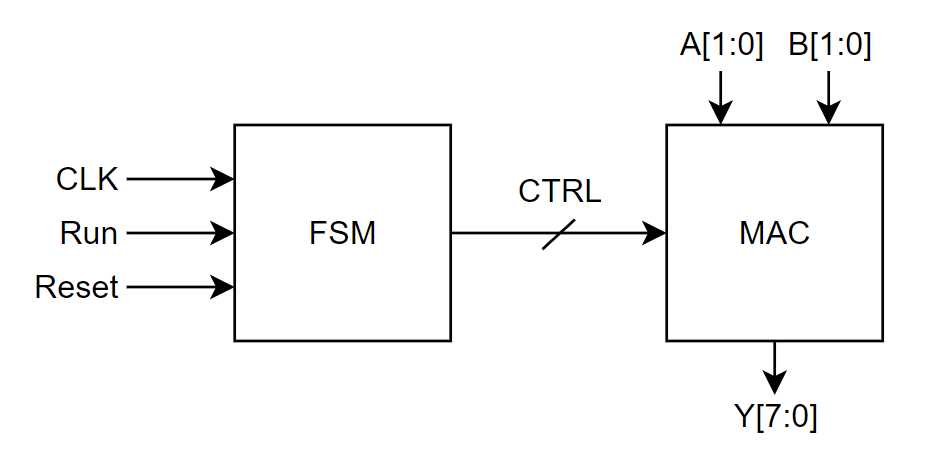
\includegraphics[width=0.7\textwidth]{Figures/Blokk.png}
    \caption{An overview of the complete system.}
    \label{fig:blokk}
\end{figure}


\subsection{Finite State Machine}
\label{subsec:fsm_theory}

A finite state machine (FSM) is a model used to describe a system with a finite number of states. It operates by transitioning from one state to another in response to inputs, following a defined set of rules. FSMs consist of:

\begin{enumerate}
    \item \textbf{States}: These represent distinct conditions or configurations that the system can be in. Transitions occur between states based on inputs.
    
    \item \textbf{Transitions}: These are directed connections between states, triggered by specific input conditions. Transitions determine the movement from one state to another.
    
    \item \textbf{Inputs}: These are external signals that trigger state transitions. Inputs influence the behavior of the FSM.
    
    \item \textbf{Outputs}: FSMs may generate outputs in response to inputs and state transitions. Outputs convey information about the current state or operation of the system.
\end{enumerate}

\noindent
FSMs can be classified into two main types:

\begin{enumerate}
    \item \textbf{Mealy Machine}: In a Mealy machine, the outputs depend on both the current state and the input. The output is produced immediately after an input is received and a state transition occurs. 
    
    \item \textbf{Moore Machine}: In a Moore machine, the outputs depend only on the current state. The output is associated with the state itself, so it changes only after a state transition.
\end{enumerate}

A general overview of the functionality is shown in figure~\ref{fig:general_fsm}.

\begin{figure}[H]
    \centering
    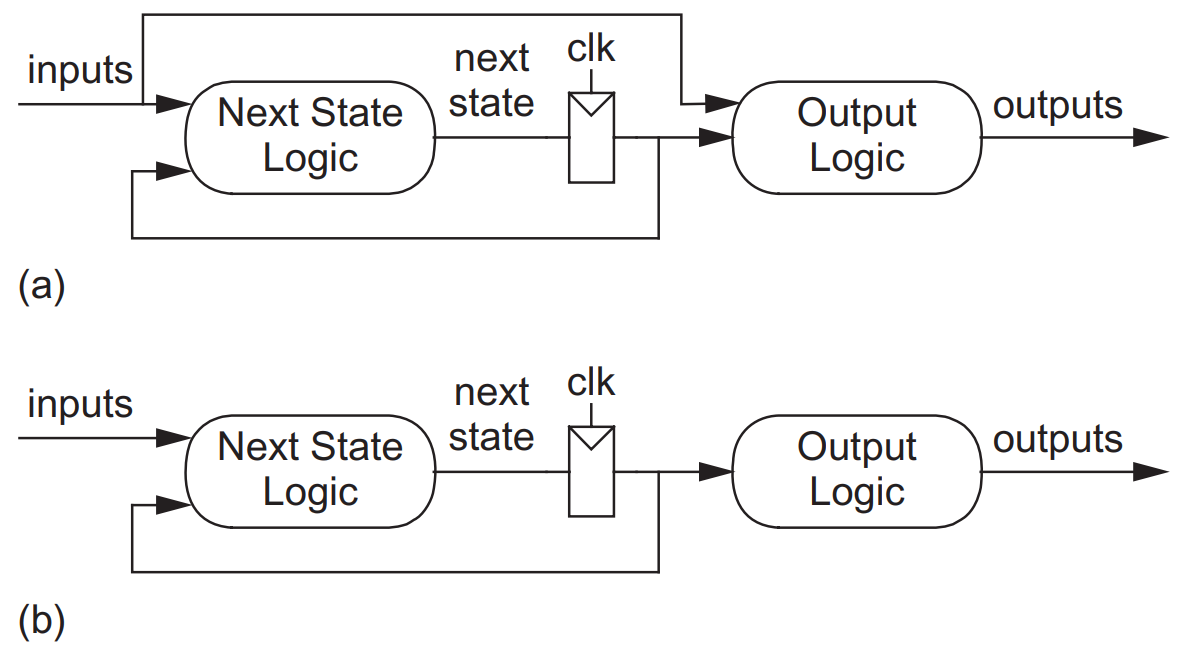
\includegraphics[width=0.8\textwidth]{Figures/general fsm diagrams.png}
    \caption{a: Mealy FSM b: Moore FSM (Figure is taken from \cite{CMOS_VLSI_design}, p.735)}
    \label{fig:general_fsm}
\end{figure}


\noindent
A certain design procedure can be used for the design of FSMs~\cite{digital_design}:

\begin{enumerate}
  \item From the word description and specifications of the desired operation, derive a state diagram for the circuit.
  \item Reduce the number of states if necessary.
  \item Assign binary values to the states.
  \item Obtain a binary-coded state table.
  \item Choose the type of flip-flops to be used.
  \item Derive the simplified flip-flop input equations and output equations.
  \item Draw the logic diagram.
\end{enumerate}


\subsection{MAC}
\label{subsec:MAC_theory}

\begin{equation}
    \label{eq:mac}
    C \leftarrow C + (A \cdot B)
\end{equation}

The MAC unit will receive two 2-bit inputs, A and B, which will be multiplied and added to C, as shown in \ref{eq:mac}. This should happen every rising edge of the clock. The MAC unit consist of a multiplier, an adder and an accumulator. The layout of the MAC is shown in figure \ref{fig:mac-blokk}. 

\begin{figure}[htpb]
    \centering
    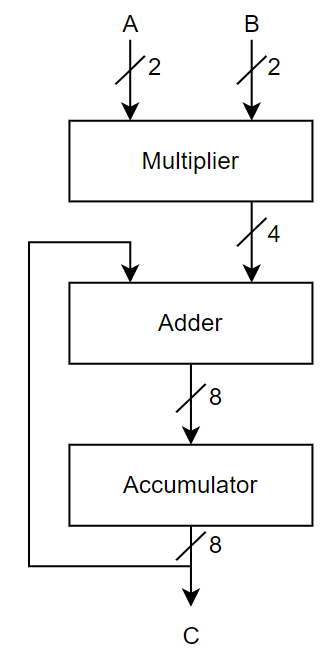
\includegraphics[width=0.3\textwidth]{Figures/mac-blokk.png}
    \caption{Layout of MAC unit}
    \label{fig:mac-blokk}
\end{figure}

\subsubsection{Multiplier}
The multiplier takes in A and B, two 2 bits inputs, and multiplies them. Since the inputs A and B are 2-bits input the value of each of them can't be higher that 3. This means that the output from the multiplier can't exceed 9 and the output of the multiplier has to be at least 4 bits. 

\subsubsection{Adder}
As shown in figure \ref{fig:mac-blokk}, the adder has to take the sum of a 4-bit number (A) and a 8-bit number (B). Since the multiplier only outputs a 4-bit number, the four most significant bits of A will always be set to low. The design of an 8-bit adder is shown in figure \ref{fig:adder-blokk}. The figure shows two 8-bit numbers A and B, and their sum S with a carry $C_O$. 

\begin{figure}[H]
    \centering
    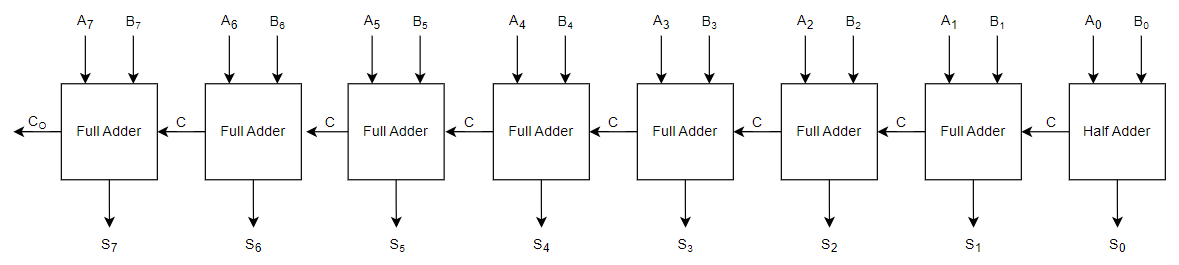
\includegraphics[width=0.8\textwidth]{Figures/8bitadder.png}
    \caption{8-bit adder}
    \label{fig:adder-blokk}
\end{figure}


\subsubsection{Accumulator}
The accumulator is an 8-bit register with some control signals, set (S) and reset (R). These controll signals are received from the Final State Machine (FSM). The registers are D-flip flops, which only change the stored value at the rising edge of the clock signal. 

\begin{figure}[H]
    \centering
    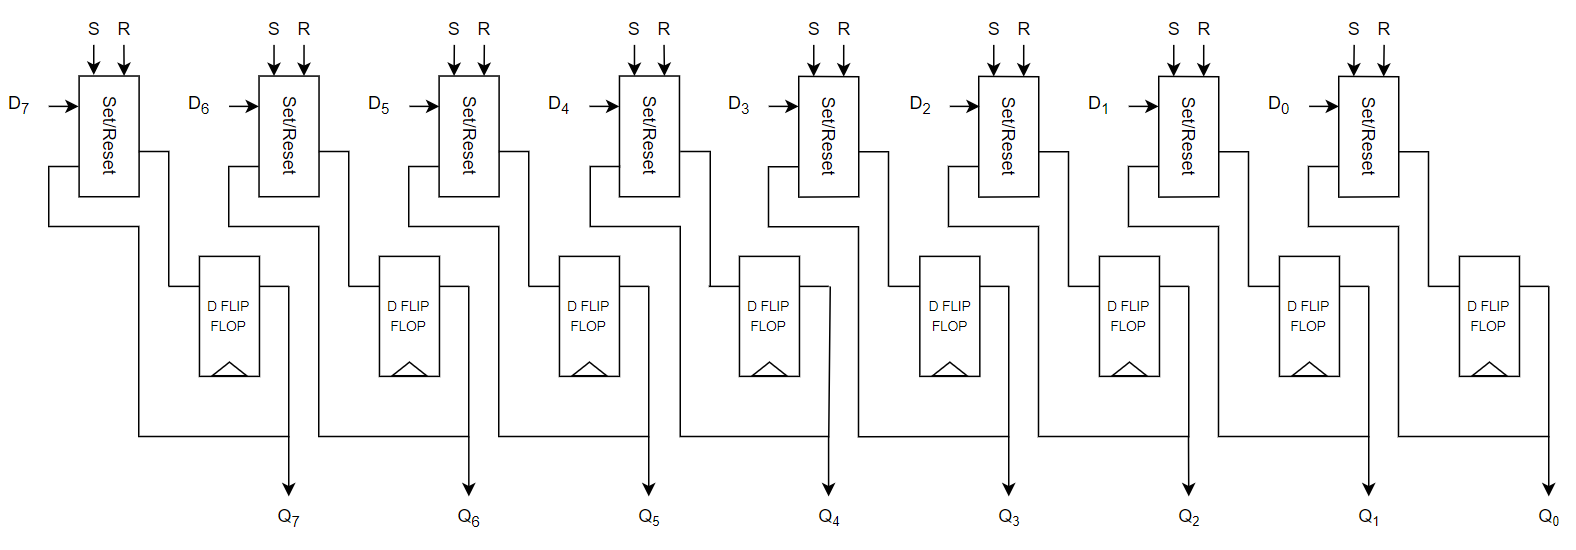
\includegraphics[width=0.9\textwidth]{Figures/8bitRegister.png}
    \caption{8 bit register}
    \label{fig:8bitregister}
\end{figure}


% The theory section should contain background theory relevant for the reader in order to understand the rest of your report. Assume that the reader is yourselves at the start of the semester (before you had learnt anything from this course) and include theory accordingly. Keep in mind that this section should only include theory relevant to the project and the report, it is not meant as a place to show off everything you have ever learnt. 

\subsection{Static Power Consumption}
\label{subsec:low_power}

One can consider many aspects of a circuit design to affect the static power consumption. Static power consumption in a circuit is primarily associated with leakage currents in transistors. The characteristics defined by a specific transistor technology as well as its width and length can influence the size of the leakage currents. As the transistor technology is given by the specifications (\ref{tab:specifications}), we may consider changing the width and length within the specifications to optimize for low leakage currents. 

In a transistor, there is three leakage currents that exists: subthreshold, gate, and
junction leakage current. Out of these the subthreshold leakage currents is in most cases the largest current. \cite{Analog_integrated} The equation for subthreshold leakage current is given by \autoref{eq:subthresholdcurrent}. 

\begin{equation}
    \label{eq:subthresholdcurrent}
    I_{D(sub-th)} \approx I_{D0}\left(\frac{W}{L}\right)e^{\left(\frac{qV_{eff}}{nkT}\right)}
\end{equation}

As we can see in \autoref{eq:subthresholdcurrent}, the width is proportional to the subthreshold leakage current and the length is inverse proportional. Therefore a smaller width and larger length can optimize the leakage current in the circuit.

Since $V_{eff} < 0$ in subthreshold region the leakage current will have a proportional relationship with the temperature. So when the temperature increases, the leakage current will increase as well. 

In an ideal scenario, one might approximate to say that the leakage current increases linearly with the number of transistors, assuming each transistor contributes an equal amount to leakage current. However, in reality, the relationship is more complex. This simplification is useful nevertheless and is used when considering design choices in this project.

When  the static power consumption for the TT and FF corner, we look at a state where the CLK is not running and the inputs, D, S and R, are set to low. The static power consumption is calculated by taking the leakage current in the $V_{DD}$ node and multiplying it with the $V_{DD}$, as shown in \autoref{eq:power}.

\begin{equation}
    \label{eq:power}
    P = I \cdot V_{DD}
\end{equation}

\subsection{Other theory}\label{subsec:theory_aSubsection}

**Insert other relevant theory here**


% When you in later sections apply any of the theory you can refer back to this section. To make it easier for the reader to understand which part you are referring back to, it can be a good idea to divide your sections into subsections (e.g. one subsection per topic). This also makes it easier to read.

% Use equations, figures and tables to help get your message across. All figures/tables/equations should be referenced in the text, as they are there to help you tell your story. Remember to cite your references \cite{example}.